The methods detailed in this paper can also be used to analyse multi-magnet systems. This section focuses on a planar Halbach array created by tessellating frustum magnets for use in planar motors. These arrays may also be used in applications such as planar magnetic loudspeakers and 3D printers. The optimisation routine will vary the geometry to not only increase field strength, but to create a \(z\)-field which closely resembles a desired profile.

\subsection{Defining array geometry}
A planar Halbach array of frustum magnets can be created by tessellating frusta of square-based pyramids and tetrahedra, shown in Figure \ref{fig:p3halbachFrustumGeometry}. Figure \ref{fig:p3halbachFrustumGeometry} shows the repeating unit for this array, which, when duplicated, creates the array shown in Figure \ref{fig:p3planarHalbach}.
\begin{figure*}
	\centering
	\def\Lpontwo{10}
\def\lpontwo{20}
\def\Ltontwo{14}
\def\ltontwo{4}
\def\hh{25}
\def\myscale{0.07}
\def\mywidth{0.3}

\begin{subfigure}[t]{\mywidth\linewidth}

\centering
\tdplotsetmaincoords{70}{35}
\begin{tikzpicture}[scale=\myscale,tdplot_main_coords]

% Define coordinates
\coordinate(1) at (-\Lpontwo,-\Lpontwo,0);
\coordinate(2) at (\Lpontwo,-\Lpontwo,0);
\coordinate(3) at (\Lpontwo,\Lpontwo,0);
\coordinate(4) at (-\Lpontwo,\Lpontwo,0);
\coordinate(5) at (-\lpontwo,-\lpontwo,-\hh);
\coordinate(6) at (\lpontwo,-\lpontwo,-\hh);
\coordinate(7) at (\lpontwo,\lpontwo,-\hh);
\coordinate(8) at (-\lpontwo,\lpontwo,-\hh);

% Draw the shape
\draw (1) -- (2) -- (3) -- (4) -- cycle;
\draw (1) -- (5) -- (6) -- (7) -- (3);
\draw[dashed] (7) -- (8) -- (5);
\draw (2) -- (6);
\draw[dashed] (4) -- (8);

\node(Lp) at (-\Lpontwo-5,3,1) {\(L_p\)};
\node(Lp2) at (0,\Lpontwo+5,1) {\(L_p\)};
\node(lp) at (\lpontwo+5,0,-\hh-1) {\(l_p\)};
\node(lp2) at (3,-\lpontwo-6,-\hh-1) {\(l_p\)};

\end{tikzpicture}

\subcaption{}
\label{subfig:p3pfrus3d}

\end{subfigure}
~
\begin{subfigure}[t]{\mywidth\linewidth}
	
\centering
\tdplotsetmaincoords{70}{35}
\begin{tikzpicture}[scale=\myscale,tdplot_main_coords]

% Define coordinates
\coordinate(1) at (-\Ltontwo,-\Lpontwo,0);
\coordinate(2) at (\Ltontwo,-\Lpontwo,0);
\coordinate(3) at (\Ltontwo,\Lpontwo,0);
\coordinate(4) at (-\Ltontwo,\Lpontwo,0);
\coordinate(5) at (-\ltontwo,-\lpontwo,-\hh);
\coordinate(6) at (\ltontwo,-\lpontwo,-\hh);
\coordinate(7) at (\ltontwo,\lpontwo,-\hh);
\coordinate(8) at (-\ltontwo,\lpontwo,-\hh);

% Draw the shape
\draw (1) -- (2) -- (3) -- (4) -- cycle;
\draw (1) -- (5) -- (6) -- (7) -- (3);
\draw[dashed] (7) -- (8) -- (5);
\draw (2) -- (6);
\draw[dashed] (4) -- (8);

\node(Lp) at (-\Ltontwo-5,3,1) {\(L_p\)};
\node(Lt) at (0,\Lpontwo+5,1) {\(L_t\)};
\node(lp) at (\ltontwo+5,0,-\hh-1) {\(l_p\)};
\node(lt) at (3,-\lpontwo-6,-\hh-1) {\(l_t\)};

\end{tikzpicture}

\subcaption{}
\label{subfig:p3tfrus3d}
	
\end{subfigure}
~
\begin{subfigure}[t]{\mywidth\linewidth}
	
	\centering
	\tdplotsetmaincoords{70}{35}
	\begin{tikzpicture}[scale=0.06,tdplot_main_coords]
	
	% Define coordinates of z frustum
	\coordinate(1z) at (-\Lpontwo,-\Lpontwo,0);
	\coordinate(2z) at (\Lpontwo,-\Lpontwo,0);
	\coordinate(3z) at (\Lpontwo,\Lpontwo,0);
	\coordinate(4z) at (-\Lpontwo,\Lpontwo,0);
	\coordinate(5z) at (-\lpontwo,-\lpontwo,-\hh);
	\coordinate(6z) at (\lpontwo,-\lpontwo,-\hh);
	\coordinate(7z) at (\lpontwo,\lpontwo,-\hh);
	\coordinate(8z) at (-\lpontwo,\lpontwo,-\hh);
	
	% Define coordinates of x frustum
	\coordinate(1x) at (\Lpontwo,-\Lpontwo,0);
	\coordinate(2x) at (\Lpontwo+\Ltontwo+\Ltontwo,-\Lpontwo,0);
	\coordinate(3x) at (\Lpontwo+\Ltontwo+\Ltontwo,\Lpontwo,0);
	\coordinate(4x) at (\Lpontwo,\Lpontwo,0);
	\coordinate(5x) at (\lpontwo,-\lpontwo,-\hh);
	\coordinate(6x) at (\lpontwo+\ltontwo+\ltontwo,-\lpontwo,-\hh);
	\coordinate(7x) at (\lpontwo+\ltontwo+\ltontwo,\lpontwo,-\hh);
	\coordinate(8x) at (\lpontwo,\lpontwo,-\hh);
	
	% Define coordinates of y frustum
	\coordinate(1y) at (-\Lpontwo,\Lpontwo,0);
	\coordinate(2y) at (\Lpontwo,\Lpontwo,0);
	\coordinate(3y) at (\Lpontwo,\Lpontwo+\Ltontwo+\Ltontwo,0);
	\coordinate(4y) at (-\Lpontwo,\Lpontwo+\Ltontwo+\Ltontwo,0);
	\coordinate(5y) at (-\lpontwo,\lpontwo,-\hh);
	\coordinate(6y) at (\lpontwo,\lpontwo,-\hh);
	\coordinate(7y) at (\lpontwo,\lpontwo+\ltontwo+\ltontwo,-\hh);
	\coordinate(8y) at (-\lpontwo,\lpontwo+\ltontwo+\ltontwo,-\hh);
	
	% Deal with certain lines behind objects
	\draw(3y) -- (7y);
	\filldraw[fill=white] (1x) -- (2x) -- (3x) -- (4x) -- cycle;
	\filldraw[fill=white] (2x) -- (3x) -- (7x) -- (6x) -- cycle;
	
	% Draw z frustum
	\draw (1z) -- (2z);
	\draw (3z) -- (4z) -- (1z);
	\draw (1z) -- (5z) -- (6z);
	\draw (2z) -- (6z);
	
	% Draw x frustum
	\draw (5x) -- (6x);
	
	% Draw y frustum
	\draw (2y) -- (3y) -- (4y) -- (1y);
	
	% Draw an invisible node to align left and right pictures
	\node(invis) at (0,0,-1.75*\hh) { };
	
	\end{tikzpicture}
	\subcaption{}
	\label{subfig:p3subarray3d}
	
\end{subfigure}

\begin{subfigure}[t]{\mywidth\linewidth}
	
	\centering
	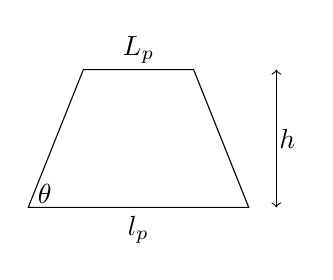
\begin{tikzpicture}[scale = \myscale]
	
	\coordinate(1) at (-\Lpontwo,0);
	\coordinate(2) at (\Lpontwo,0);
	\coordinate(5) at (-\lpontwo,-\hh);
	\coordinate(6) at (\lpontwo,-\hh);
	
	\draw (1) -- (2) -- (6) -- (5) -- cycle;
	\node(theta) at (-\lpontwo+3,-\hh+2.5) {\(\theta\)};
	\node(Lp) at (0,3.5) {\(L_p\)};
	\node(lp) at (0,-\hh-4) {\(l_p\)};
	\draw[<->] (\lpontwo+5,-\hh) -- (\lpontwo+5,0);
	\node(h) at (\lpontwo+7,-12.5) {\(h\)};
	
	\end{tikzpicture}
	
	\subcaption{}
	\label{subfig:p3pfrusschematic}
	
\end{subfigure}
~
\begin{subfigure}[t]{\mywidth\linewidth}
	
\centering
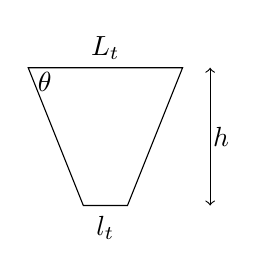
\begin{tikzpicture}[scale = \myscale]

\coordinate(1) at (-\Ltontwo,0);
\coordinate(2) at (\Ltontwo,0);
\coordinate(5) at (-\ltontwo,-\hh);
\coordinate(6) at (\ltontwo,-\hh);

\draw (1) -- (2) -- (6) -- (5) -- cycle;
\node(theta) at (-\Ltontwo+3,-2.5) {\(\theta\)};
\node(Lp) at (0,3.5) {\(L_t\)};
\node(lp) at (0,-\hh-4) {\(l_t\)};
\draw[<->] (\Ltontwo+5,-\hh) -- (\Ltontwo+5,0);
\node(h) at (\Ltontwo+7,-12.5) {\(h\)};

\end{tikzpicture}

\subcaption{}
\label{subfig:p3tfrusschematic}
	
\end{subfigure}
~
\begin{subfigure}[t]{\mywidth\linewidth}
	
	\centering
	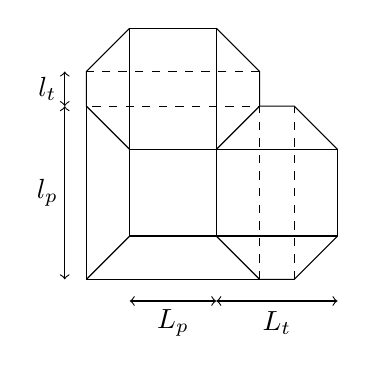
\begin{tikzpicture}[scale=0.055]
	
	% Define coordinates of z frustum
	\coordinate(1z) at (-\Lpontwo,-\Lpontwo);
	\coordinate(2z) at (\Lpontwo,-\Lpontwo);
	\coordinate(3z) at (\Lpontwo,\Lpontwo);
	\coordinate(4z) at (-\Lpontwo,\Lpontwo);
	\coordinate(5z) at (-\lpontwo,-\lpontwo);
	\coordinate(6z) at (\lpontwo,-\lpontwo);
	\coordinate(7z) at (\lpontwo,\lpontwo);
	\coordinate(8z) at (-\lpontwo,\lpontwo);
	
	% Define coordinates of x frustum
	\coordinate(1x) at (\Lpontwo,-\Lpontwo);
	\coordinate(2x) at (\Lpontwo+\Ltontwo+\Ltontwo,-\Lpontwo);
	\coordinate(3x) at (\Lpontwo+\Ltontwo+\Ltontwo,\Lpontwo);
	\coordinate(4x) at (\Lpontwo,\Lpontwo);
	\coordinate(5x) at (\lpontwo,-\lpontwo);
	\coordinate(6x) at (\lpontwo+\ltontwo+\ltontwo,-\lpontwo);
	\coordinate(7x) at (\lpontwo+\ltontwo+\ltontwo,\lpontwo);
	\coordinate(8x) at (\lpontwo,\lpontwo);
	
	% Define coordinates of y frustum
	\coordinate(1y) at (-\Lpontwo,\Lpontwo);
	\coordinate(2y) at (\Lpontwo,\Lpontwo);
	\coordinate(3y) at (\Lpontwo,\Lpontwo+\Ltontwo+\Ltontwo);
	\coordinate(4y) at (-\Lpontwo,\Lpontwo+\Ltontwo+\Ltontwo);
	\coordinate(5y) at (-\lpontwo,\lpontwo);
	\coordinate(6y) at (\lpontwo,\lpontwo);
	\coordinate(7y) at (\lpontwo,\lpontwo+\ltontwo+\ltontwo);
	\coordinate(8y) at (-\lpontwo,\lpontwo+\ltontwo+\ltontwo);
	
	% Draw top plane
	\draw (1z) -- (2z) -- (3z) -- (4z) -- cycle;
	\draw (2y) -- (3y) -- (4y) -- (1y);
	\draw (1x) -- (2x) -- (3x) -- (4x);
	
	% Draw connecting planes where necessary
	\draw (1z) -- (5z);
	\draw (1x) -- (5x) -- (6x) -- (2x);
	\draw (3x) -- (7x) -- (8x) -- (4x);
	\draw (6y) -- (7y) -- (3y);
	\draw (1y) -- (5y) -- (8y) -- (4y);
	
	% Draw bottom plane
	\draw (8z) -- (5z) -- (6z);
	\draw[dashed] (6z) -- (7z) -- (8z);
	\draw[dashed] (7y) -- (8y);
	\draw[dashed] (6x) -- (7x);
	
	% Draw some dimensions
	\draw[<->] (-\Lpontwo,-\lpontwo-5) -- (\Lpontwo,-\lpontwo-5);
	\draw[<->] (\Lpontwo,-\lpontwo-5) -- (\Lpontwo+2*\Ltontwo,-\lpontwo-5);
	\draw[<->] (-\lpontwo-5,-\lpontwo) -- (-\lpontwo-5,\lpontwo);
	\draw[<->] (-\lpontwo-5,\lpontwo) -- (-\lpontwo-5,\lpontwo+2*\ltontwo);
	\node(Lp) at (0,-\lpontwo-10) {\(L_p\)};
	\node(Lt) at (\Lpontwo+\Ltontwo,-\lpontwo-10) {\(L_t\)};
	\node(lp) at (-\lpontwo-9,0) {\(l_p\)};
	\node(lt) at (-\lpontwo-9,\lpontwo+\ltontwo) {\(l_t\)};
	
	\end{tikzpicture}
	\subcaption{}
	\label{subfig:p3subarrayschematic}
	
\end{subfigure}


	\caption{Three dimensional views and schematics of a pyramid frustum (\subref{subfig:p3pfrus3d},\subref{subfig:p3pfrusschematic}), a tetrahedral frustum (\subref{subfig:p3tfrus3d},\subref{subfig:p3tfrusschematic}), and the repeating unit (\subref{subfig:p3subarray3d},\subref{subfig:p3subarrayschematic}).}
	\label{fig:p3halbachFrustumGeometry}
\end{figure*}
\begin{figure}
	\centering
	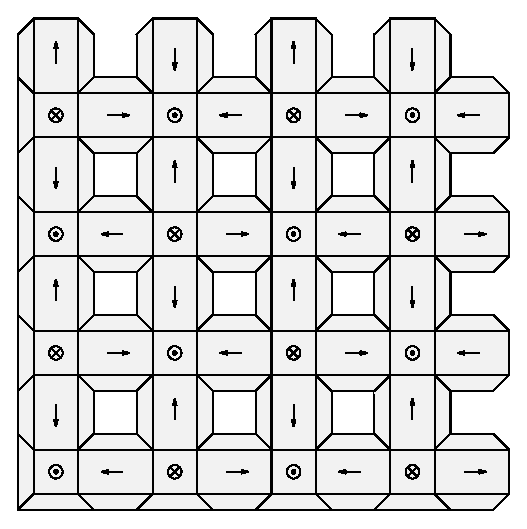
\includegraphics[width=0.7\linewidth]{p3/p3FIG11}
	\caption{Planar Halbach array created by replicating the magnetic subarray from Figure \ref{fig:p3halbachFrustumGeometry}. The pyramid frusta have magnetisations in the \(z\)-direction (into and out of the page), whereas the tetrahedral frusta have magnetisations in the \(x\)- and \(y\)-directions (parallel to the page).}
	\label{fig:p3planarHalbach}
\end{figure}

The square-based pyramid frustum (Figure \ref{fig:p3squareFrustum}) requires three parameters to fully describe its geometry, while the tetrahedral frustum requires five parameters, totalling eight parameters. However, for the magnets to tessellate, two of the length parameters (\(l_p\) and \(L_p\)), the wall angle \(\theta\), and height \(h\) are shared between the two, leaving only four parameters required to fully describe the system geometry. This is reduced to two parameters by keeping the system volume and pole pitch \(\tau\) constant.

Consider the repeating unit shown in Figure \ref{fig:p3halbachFrustumGeometry} (\subref{subfig:p3subarray3d} and \subref{subfig:p3subarrayschematic}) with the magnets having an average volume \(V\). Let the total volume of the three magnets be \(3V\) units\(^3\) and the pole pitch be \(\tau = L_p + L_t = l_p + l_t\) units. Define the parameters \(h\) and \(\theta\) as variables. Thus, the geometry is fully defined by the relations
\begin{align}
l_p &= \tau + h \cot \theta - S \\ 
L_p &= \tau - h \cot \theta - S \\
l_t &= -h \cot \theta + S \\
L_t &= h \cot \theta + S \text{,}
\end{align}
where
\begin{equation}
S = \sqrt{\tau^2 - \frac{3V}{h} - \frac{h^2}{3} \cot^2\theta} \text{.}
\end{equation}
Therefore, for constant \(V\) and \(\tau\), the array geometry can be fully described using the variables \(h\) and \(\theta\).

\subsection{Optimisation of field for a specific case}\label{sec:p3specificOptimisation}
Consider an array using a repeating unit with length \(\tau/\upsilon = 2\) for use in a planar motor with low force ripple and large maximum force. Selection of a suitable desired field profile depends on coil geometry specific to each motor, but this work considers only permanent magnet geometry, and as such a general sinusoidal profile is chosen as the desired \(z\)-field profile. Further extensions of this work could consider a field profile tailored to a particular motor design. Although force ripple will not be completely removed using a sinusoidal profile, it will be reduced when compared to the field produced by a traditional cuboidal array. In addition, a field profile with a large amplitude will lead to a larger maximum force for the motor. Thus, a sinusoid with large amplitude is chosen as the desired field profile for the optimisation routine. Both the resemblance and amplitude can be quantified using a least squares analysis on calculated field data and the appropriate two-dimensional cosine wave \(f\), given by
\begin{equation}\label{eqn:p3cosineWave}
f\left(x,y\right) = A\cos\left(\frac{\pi x}{\tau}\right)\cos\left(\frac{\pi y}{\tau}\right) \text{,}
\end{equation}
where \(A\) is the amplitude of the sinusoid.

For a given geometry \(\left(h/\upsilon,\theta\right)\) and vertical distance \(z/\upsilon\) from the array, the \(z\)-field was calculated over a \(2\tau/\upsilon\times2\tau/\upsilon\) region across a \(32\times32\) grid of points to include one full wavelength of the magnetic field. This calculation was done using five pole pitches in each direction, giving a large enough array such that end effects were negligible, but maintaining a relatively small calculation time. At each point, \(f\) was calculated, and the sum of squared residuals minimised to give the value of the wave amplitude \(A\). The coefficient of determination \(r^2\) was calculated, giving a measure of similarity between the field data and cosine wave. This process was repeated for a large range of geometries \(\left(\theta, h/\upsilon\right)\), and contour plots drawn for \(r^2\) and \(A\). These plots show the optimal regions to maximise \(r^2\) or \(A\), and are shown for \(z/\upsilon = 0.2\) in Figure \ref{fig:p3planarHalbachData}.
\begin{figure}
	\centering
	\begin{subfigure}{0.8\textwidth}
		\centering
		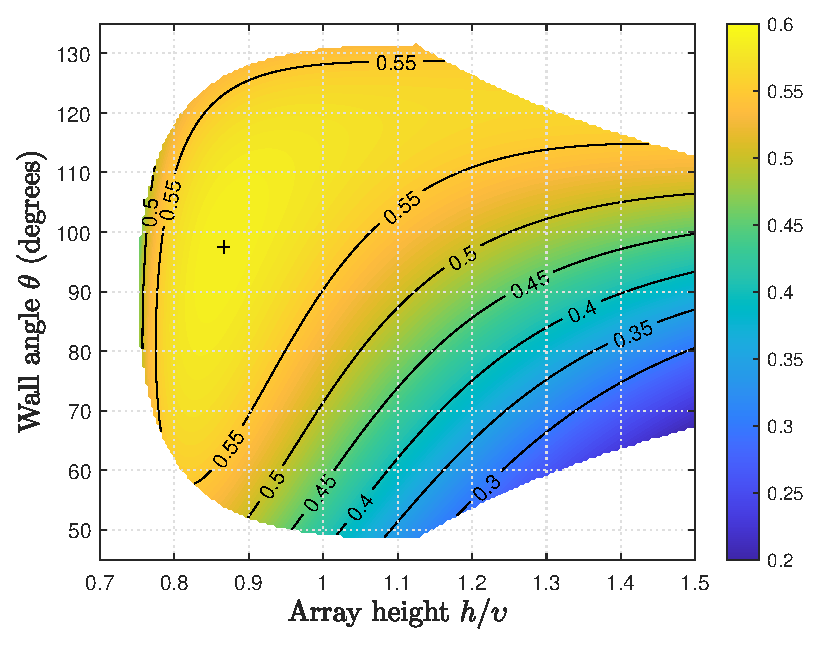
\includegraphics[width=\linewidth]{p3/p3FIG12a}
		\subcaption{}
		\label{subfig:p3planarHalbach_amp}
	\end{subfigure}
	
	\vfill
	
	\begin{subfigure}{0.8\textwidth}
		\centering
		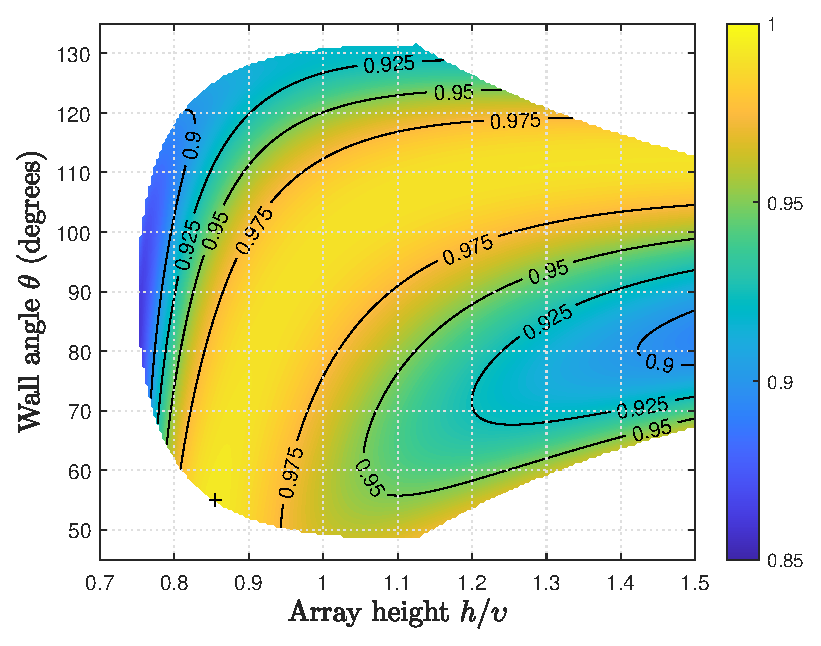
\includegraphics[width=\linewidth]{p3/p3FIG12b}
		\subcaption{}
		\label{subfig:p3planarHalbach_rsq}
	\end{subfigure}
	\caption{Normalised amplitude \(A\) (\subref{subfig:p3planarHalbach_amp}) and coefficient of determination \(r^2\) (\subref{subfig:p3planarHalbach_rsq}) of the cosine wave approximation of the \(z\)-field above the planar magnet array with \(\tau/\upsilon=2\) and \(z/\upsilon = 0.2\). The global maxima are plotted with a `+', with the white region indicating non-physical geometries.}
	\label{fig:p3planarHalbachData}
\end{figure}

The contour plots indicated that there are relatively large regions which maximise \(r^2\) and \(A\). The region to maximise \(r^2\) is a curved stripe, starting with low \(\theta\) and \(h/\upsilon\), passing through the cube case (\(\theta = \) \ang{90}, \(h/\upsilon = 1\)), and tending toward large \(\theta\) and \(h/\upsilon\). The region to maximise \(A\) is a triangular area in the top left of the plot. There is overlap between the optimal regions of both plots along the bottom edge of the optimal region of \(A\) and the top edge of the optimal region of \(r^2\). Hence, the geometry to maximise both \(r^2\) and \(A\) will be in this overlap region.

This can be further examined by defining a cost function to maximise both,
\begin{equation}\label{eqn:p3CostFunction}
C = Ar^2 \text{.}
\end{equation}

Maximising \(C\) will give large values for both \(r^2\) and \(A\), thereby obtaining a field which closely resembles a cosine wave with large amplitude. The cost function \(C\) was calculated at each combination \(\left(\theta, h/\upsilon\right)\) (Figure \ref{fig:p3planarHalbach_wavequality}). This plot shows a region coinciding with the overlap of Figures \ref{subfig:p3planarHalbach_rsq} and \ref{subfig:p3planarHalbach_amp} as expected. The maximum value of this plot occurs at \(h_\text{opt}/\upsilon = 0.89\) and \(\theta_\text{opt} =\) \ang{93.3}. This geometry is almost cuboidal, and thus corresponds to an increase of only 0.04\% in \(C\) over the optimal cuboidal geometry.
\begin{figure}
	\centering
	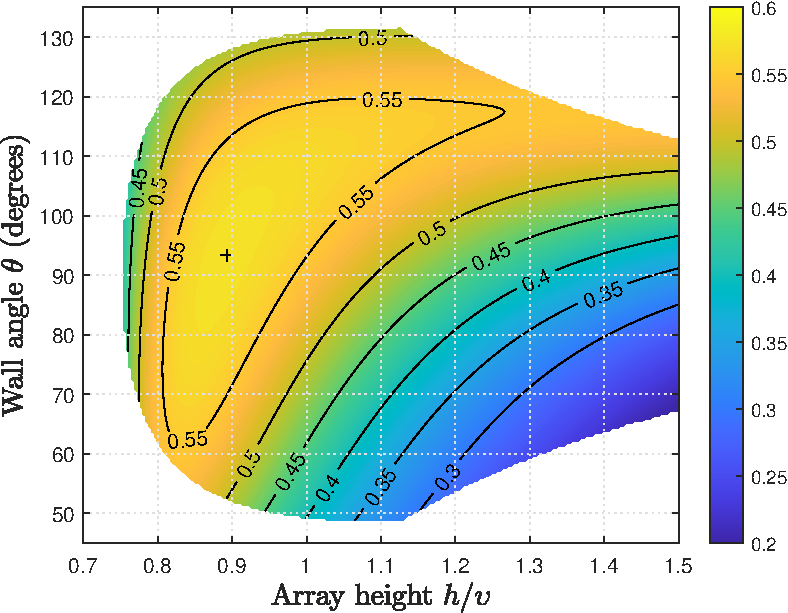
\includegraphics[width=0.8\linewidth]{p3/p3FIG13}
	\caption{The value of the cost function \(C = Ar^2\) at each point in the physically realisable region with \(\tau/\upsilon=2\) and \(z/\upsilon = 0.2\). This value is maximised in the top-left area of the region, with optimal parameters of \(h_\text{opt}/\upsilon = 0.89\) and \(\theta_\text{opt} = \) \ang{93.3}.}
	\label{fig:p3planarHalbach_wavequality}
\end{figure}

\subsection{Optimisation of field for a general case}
The methodology outlined in Section \ref{sec:p3specificOptimisation} can be extended to consider more general cases. However, rather than evaluating the value of \(C\) at each feasible geometry \(\left( \theta, h/\upsilon \right)\), an optimisation routine is used, substantially reducing the number of evaluations of \(C\). Additionally, all length parameters can be normalised by \(z\), allowing a nondimensional analysis, leading to a more general solution.

A range of values were defined for \(\upsilon/z\) and \(\tau/z\), and limits on geometries imposed to discard geometries with extreme aspect ratios. For each combination \(\left( \upsilon/z, \tau/z\right)\), the region of physically realisable geometries was identified in terms of \(h/z\) and \(\theta\). The Matlab function \texttt{fmincon} was then used to maximise the cost function \(C\) over the physically realisable magnet geometries \(\left(\theta, h/z\right)\). This process was repeated for each combination \(\left( \upsilon/z, \tau/z\right)\), and the results plotted on the contour plots in Figure \ref{fig:p3optvalues}, with the corresponding value of the cost function \(C\) plotted in Figure \ref{fig:p3generalPlanarHalbachQuality}.
\begin{figure}
	\centering
	\begin{subfigure}{0.8\textwidth}
		\centering
		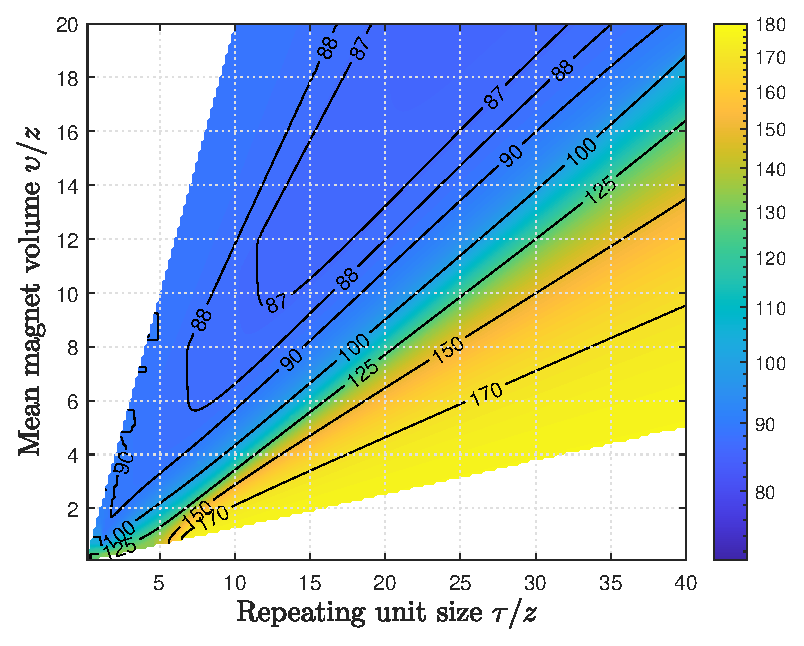
\includegraphics[width=\linewidth]{p3/p3FIG14a}
		\subcaption{}
		\label{subfig:p3opttheta}
	\end{subfigure}
	
	\begin{subfigure}{0.8\textwidth}
		\centering
		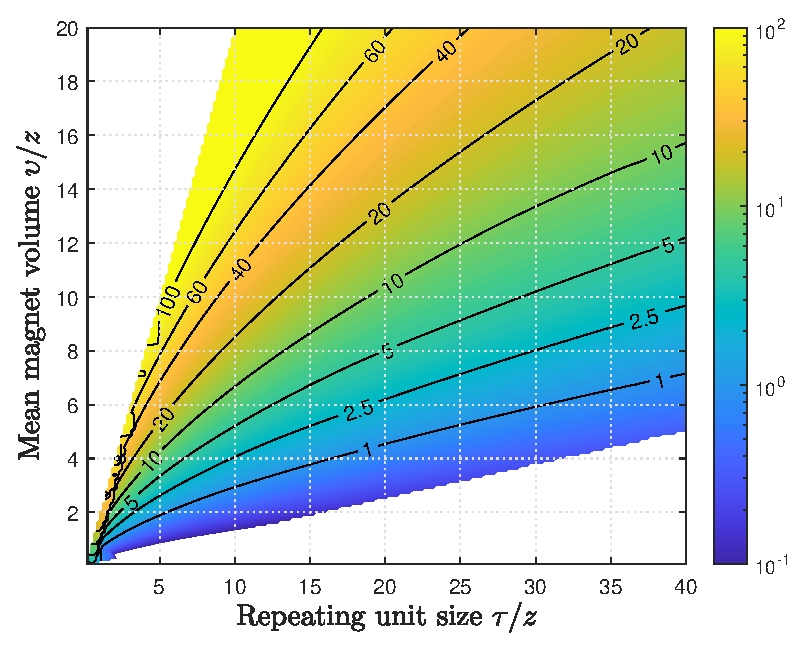
\includegraphics[width=\linewidth]{p3/p3FIG14b}
		\subcaption{}
		\label{subfig:p3opth}
	\end{subfigure}
	\caption{The optimal value of \(\theta\) (\subref{subfig:p3opttheta}) and \(h/z\) (\subref{subfig:p3opth}) for a given combination \(\left( \upsilon/z, \tau/z \right)\). The white regions indicate magnet topologies with undesirable aspect ratios.}
	\label{fig:p3optvalues}
\end{figure}
\begin{figure}
	\centering
	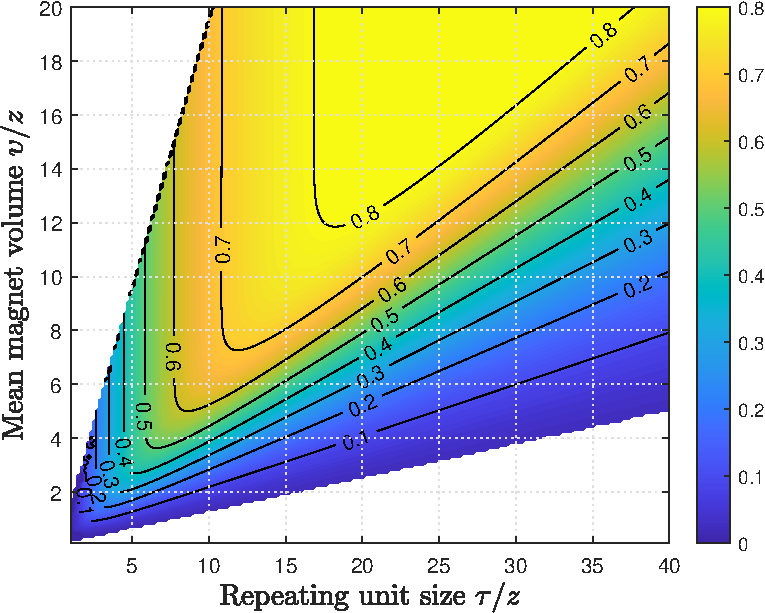
\includegraphics[width=0.8\linewidth]{p3/p3FIG15}
	\caption{The value of the cost function \(C = Ar^2\) at each combination \(\left( \upsilon/z, \tau/z \right)\) normalised by the magnetisation strength of the magnets. This value approaches unity for large \(\tau/z\) and \(\upsilon/z\), and becomes small when either \(\tau/z\) or \(\upsilon/z\) are small.}
	\label{fig:p3generalPlanarHalbachQuality}
\end{figure}

Interestingly, the upper half of the plots indicate a magnet geometry close to a cuboid. However, as the volume decreases or pole pitch increases, the optimal angle \(\theta\) grows larger, leading to a highly non-cuboidal geometry. The optimal height parameter behaves as would be expected, with increasing height as the volume increases or pole pitch decreases.

The optimal frustum topologies can be directly compared to the corresponding cuboidal topologies. The optimisation routine was run again, but this time only optimising the height parameter while maintaining the angle \(\theta\) at \ang{90}. The cost function \(C_\text{cuboid}\) was calculated and compared to the associated frustum cost function \(C\). The percentage increase in \(C\) produced by the optimal frustum over optimal cuboid was plotted for each combination \(\left( \upsilon/z, \tau/z \right)\) and is shown in Figure \ref{fig:p3percentageIncrease}, showing a small but nonzero increase in field quality.
\begin{figure}
	\centering
	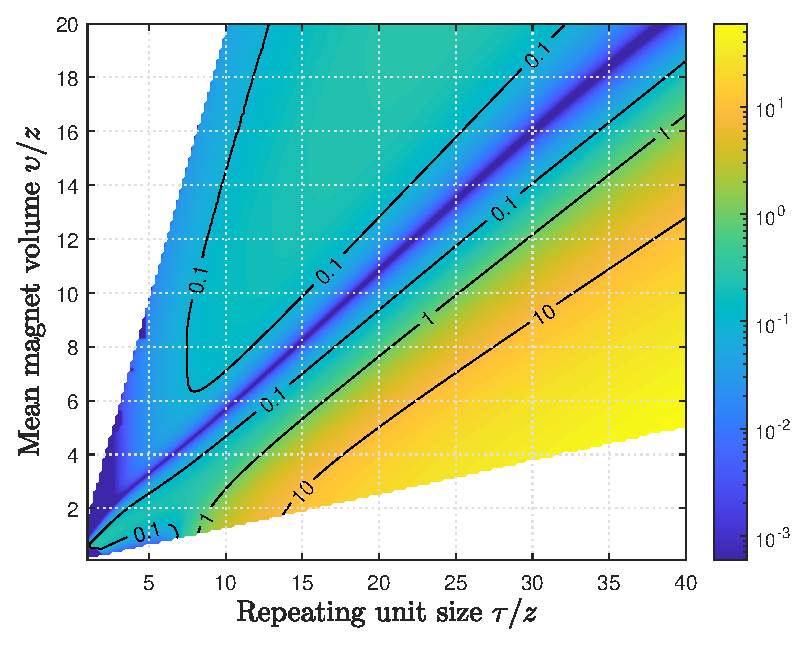
\includegraphics[width=0.8\linewidth]{p3/p3FIG16}
	\caption{Percentage increase in the cost function \(C\) using optimal frustum magnets rather than optimal cuboid magnets. In the centre of the region, the percentage increase is extremely small, implying no effective increase in performance using optimal frusta instead of optimal cuboids. In some regions, this percentage increase is larger. However, these are regions where the cost function is relatively small whether using frusta or cuboids, so it is likely more effective to redesign the system than to optimise magnet geometry.}
	\label{fig:p3percentageIncrease}
\end{figure}

In most of the region, this increase is less than 1 percent, meaning the increased difficulty and cost associate with manufacturing frustum magnets rather than cuboidal magnets is likely not worth the small increase in \(C\). The bottom right region of the plot shows a more considerable percentage increase, achieving an increase greater than 10\%. However, there are two main issues with this region. Firstly, the magnets will exhibit an extremely undesirable aspect ratio. Based on Figure \ref{subfig:p3opth}, this region has a relatively small optimal height parameter \(h/z\) in a region with large \(\tau/z\), leading to a large value of \(\tau/h\) and an undesirable aspect ratio of the magnets. Secondly, this region attains a relatively low value of \(C\) according to Figure \ref{fig:p3generalPlanarHalbachQuality}. This is partially because the magnets are very thin due to the large value of \(\tau/h\), leading to weak fields, and partially because the ratio \(\tau/z\) is large, leading to the field resembling a square wave rather than a sinusoid. These tendencies lead to a small field amplitude \(A\), with a low coefficient of determination \(r^2\), leading to a small value of \(C\).

Based on Figure \ref{fig:p3percentageIncrease}, optimal frustum magnets are likely not worth the additional difficulty and cost associated with manufacturing and assembly for a planar Halbach array. The increase in field amplitude and resemblance to a sinusoid are negligible in most regions. In the region where the increase is not insignificant, the amplitude and resemblance to a sinusoid are small independent of the magnet shape. In this region, it is likely better to redesign the system to increase the magnet volume or decrease the pole pitch of the array. In general, optimal cuboidal magnets are likely the most effective solution for a planar Halbach array which aims to attain a sinusoidal magnetic field with a large amplitude.